\documentclass[sigconf, review, anonymous]{acmart}

\usepackage{listings}
\usepackage{xcolor}

\lstset{
  basicstyle=\ttfamily\small,
  keywordstyle=\color{blue},
  commentstyle=\color{gray},
  breaklines=true,
  frame=single,
}

\AtBeginDocument{%
  \providecommand\BibTeX{{%
    Bib\TeX}}}

\setcopyright{acmlicensed}
\copyrightyear{2026}
\acmYear{2026}

\acmConference[PACT '26]{International Conference on Parallel
  Architectures and Compilation Techniques}{October 19--22,
  2026}{Chicago, IL, USA}
\acmYear{2026}
\acmISBN{}
\acmDOI{}

\begin{document}

\title{Sparse Matrix Multiply: Heterogeneous Block Format Selection via Analytical Cost Models}

\author{Spencer Smith}
\affiliation{%
  \institution{University of Oklahoma}
  \city{Norman, Oklahoma}
  \country{United States}}
\email{spencer.smith-1@ou.edu}

\author{Moez Khan}
\affiliation{%
  \institution{University of Oklahoma}
  \city{Norman, Oklahoma}
  \country{United States}}
\email{moezdurrani@ou.edu}

\author{Richard Veras}
\affiliation{%
  \institution{University of Oklahoma}
  \city{Norman, Oklahoma}
  \country{United States}}
\email{richard.m.veras@ou.edu}

\begin{abstract}
Sparse matrix-matrix multiplication (SpGEMM) is an important, performance-critical operation in
many scientific and graph workloads, yet existing implementations rarely exploit fine-grained
structural sparsity within the multiply itself, often focusing on a
global compression strategy. In this work, we present a
comprehensive benchmarking and instrumentation study of SpGEMM across a variety
of storage formats, covering all permutations of input format pairings
with dense output. Through runtime performance benchmarking and instrumentation,
we observe the floating-point operation (FLOP) and memory operation (memop) counts
for each format combination and derive analytical formulas that accurately approximate
these costs as a function of matrix density and dimensions.

With these findings, we introduce a BLIS-inspired sparse matrix multiplication algorithm
that preserves the hierarchical loop ordering and blocking of BLIS while replacing
the innermost micro-kernel with heterogeneous format sparse blocks drawn from
the aforementioned four formats. We formulate the selection of per-block formats as
an integer non-linear optimization problem, using the derived cost formulas to identify the
globally optimal format assignment for a given combination of input matrices and
their respective density distribution over the micro-blocks. We evaluate the approach
on synthetic banded diagonal matrices and real Kronecker graph datasets,
finding that block dispatch overhead dominates runtime in both cases, outweighing
the benefits of heterogeneous format selection.
\end{abstract}

\begin{CCSXML}
<ccs2012>
   <concept>
       <concept_id>10003752.10003809</concept_id>
       <concept_desc>Theory of computation~Design and analysis of algorithms</concept_desc>
       <concept_significance>300</concept_significance>
       </concept>
   <concept>
       <concept_id>10010147.10010148.10010149.10010161</concept_id>
       <concept_desc>Computing methodologies~Optimization algorithms</concept_desc>
       <concept_significance>500</concept_significance>
       </concept>
   <concept>
       <concept_id>10010147.10010169.10010170</concept_id>
       <concept_desc>Computing methodologies~Parallel algorithms</concept_desc>
       <concept_significance>300</concept_significance>
       </concept>
 </ccs2012>
\end{CCSXML}

\ccsdesc[300]{Theory of computation~Design and analysis of algorithms}
\ccsdesc[500]{Computing methodologies~Optimization algorithms}
\ccsdesc[300]{Computing methodologies~Parallel algorithms}

\keywords{Sparse,Optimization,Cost-Model,COO,CSR,CSC,SpGEMM}

\received{30 April 2026}

\maketitle

\section{Introduction}

Sparse matrix-matrix multiplication (SpGEMM) is a foundational operation in graph
analytics, scientific simulation, and machine learning, yet it remains one of the more
difficult kernels to optimize, in part due to its irregularity. Most existing high-performance
SpGEMM implementations choose a single compressed storage format globally and apply
it uniformly across the entire matrix. This ignores the fact that real-world sparse
matrices often exhibit highly non-uniform sparsity structure, that is, some regions may be
nearly dense while others are extremely sparse, and that different storage formats
could potentially have meaningfully different performance characteristics depending on
local density and the mix.

In this work, we ask whether exploiting this fine-grained structural heterogeneity can
yield performance benefits. Specifically, we investigate a block-level approach
inspired by the BLIS dense matrix multiplication framework~\cite{blis}, in which each
micro-block of the input matrices is independently assigned one of four storage
formats, Dense, CSR, CSC, or COO, based on its local density.

To support this, we first conduct a comprehensive benchmarking and instrumentation
study of SpGEMM across all sixteen pairings of these four formats with dense output.
We derive analytical formulas for floating-point and memory operation counts as a
function of both matrix dimensions and density, validating them against actual
observed, empirical counts across a sweep of input densities.
We then formulate format selection as a Mixed Integer Nonlinear Program (MINLP)
using these cost formulas and evaluate the resulting
heterogeneous format assignments against uniform-format baselines on both synthetic
banded diagonal matrices and real Kronecker graph datasets~\cite{kronecker}.

Our findings are primarily negative but informative: block dispatch overhead dominates
runtime in both test cases, outweighing any savings from heterogeneous format
selection. The cost formulas, while accurate predictors of operation counts, are poor
proxies for actual runtime at small block sizes where cache effects and branch
misprediction dominate. We discuss the conditions under which this approach might
become viable and directions for future work.

\section{Background}

\subsection{Sparse Matrix Storage Formats}
The four formats considered in this work represent the standard vocabulary of sparse
matrix storage. Compressed Sparse Row (CSR) stores non-zeros row by row, with a row
pointer array enabling efficient traversal of row entries.
Compressed Sparse Column (CSC) is the column-major analog: columns are stored
contiguously, making it efficient for column-wise access patterns. Coordinate format
(COO) stores each non-zero as an explicit $(\text{row}, \text{col}, \text{value})$
triple, meaning pointer compression but consuming more memory per entry and
imposing a scan cost proportional to the total non-zero count during row-wise access.
Dense format stores all elements explicitly in a flat row-major array, eliminating
indexing overhead entirely and exposing maximum memory locality, making it optimal
when most entries are non-zero, unsurprisingly. Each format encodes the same mathematical
object but makes different trade-offs between storage overhead,
access pattern regularity, and the cost of skipping structural zeros.
The standard reference for these formats in the context of sparse linear algebra
compilers is \cite{taco_formats}, who provide a unified description of
format capabilities in terms of per-dimension storage modes.

\subsection{SpGEMM}
SpGEMM computes $C = A \times B$ where $A$ and $B$ are sparse matrices. Unlike sparse
matrix-vector multiplication (SpMV), SpGEMM involves two sparse operands whose
non-zero structure interacts during multiplication: the output sparsity pattern is not
known in advance and must be computed symbolically before numeric accumulation can
begin. The operation appears as a core subroutine in algebraic multigrid solvers,
triangle counting, multi-source breadth-first search, and high-dimensional similarity
search, among many other applications~\cite{spgemm_survey}.
Buluç and Gilbert~\cite{buluc_gilbert}
provide foundational parallel algorithms for SpGEMM.
The most performance-relevant observation for this work is that SpGEMM is overwhelmingly
memory-bound on current hardware: the irregular, format-dependent access patterns of
sparse operands generate large numbers of short, unpredictable memory requests, keeping
arithmetic units underutilized.

\subsection{BLIS}
The BLAS-like Library Instantiation Software (BLIS) framework~\cite{blis} provides a
portable infrastructure for implementing dense level-3 BLAS operations. Its key insight
is that virtually all computation in dense matrix multiplication can be expressed in
terms of a small, hardware-specific micro-kernel operating on dense register-sized
panels, surrounded by a fixed five-loop blocking structure parameterized by cache-level
constants $m_c$, $n_c$, $k_c$ and micro-kernel block sizes $m_r$ and $n_r$. This
separation allows the bulk of the framework to be written once in portable C while
performance-critical sections are tuned per architecture. Our implementation preserves
this five-loop structure and blocking hierarchy, replacing only the innermost
micro-kernel with a dispatch over heterogeneous sparse formats.

\subsection{Roofline Model}
The roofline model~\cite{roofline} provides an upper bound on achievable kernel
performance as a function of arithmetic intensity (FLOPs per byte of memory traffic).
For a given kernel and machine, the model draws a ``roofline'' as the minimum of the
peak compute throughput and the product of memory bandwidth and arithmetic intensity. A
kernel is compute-bound if its arithmetic intensity exceeds the machine's
compute-to-bandwidth ratio, and memory-bound otherwise. SpGEMM kernels consistently
fall in the memory-bound regime due to low data reuse and irregular access patterns, a
finding confirmed by our results in Section 4.

\subsection{TACO}
The Tensor Algebra Compiler (TACO)~\cite{taco} automatically generates efficient
kernels for any compound tensor algebra expression over mixed dense and sparse tensors,
including all format combinations relevant to this work. TACO provides a principled
formalization of how iteration spaces and index expressions vary across storage formats,
and its generated kernels served as the starting point and correctness reference for our
hand-instrumented implementations.

\subsection{Kronecker Graphs}
Kronecker graphs~\cite{kronecker} are a family of self-similar synthetic networks
generated by repeated Kronecker product of a small initiator matrix with itself. They
were introduced as a model for real-world networks because their recursive structure
naturally produces the heavy-tailed degree distributions and small diameters observed
in internet topology graphs and social networks. The AS-Newman autonomous systems
dataset used in our experiments is a standard benchmark graph commonly represented as
a Kronecker graph instance.

\subsection{Optimization}
Format selection in this work is formulated as a Mixed Integer Nonlinear Program
(MINLP) and solved using Pyomo~\cite{pyomo} with MindtPy~\cite{mindtpy} as the MINLP
solver back-end, using GLPK for MIP subproblems and IPOPT for the NLP relaxations.

\section{Mechanism / Methodology}

\subsection{Instrumentation and Benchmarking}
Each matrix multiplication kernel was initially derived using the TACO compiler as a reference,
then rewritten by hand to incorporate a custom instrumentation layer. Each kernel is
itself actually implemented as a C preprocessor macro, allowing the same implementation
to be invoked both within the benchmarking framework and directly as a callable
function in the sparse BLIS multiplication pipeline. The instrumentation layer is then
built on top of this using a second set of macros, \texttt{LOAD}, \texttt{STORE},
and \texttt{FMADD}, which in their counting mode expand to the underlying operation
plus a bit of bookkeeping to record memory and floating point operation activity.
Each \texttt{FMADD} increments a floating point operation counter by two, while
each \texttt{LOAD} and \texttt{STORE} increments both a memory operation counter and a
byte counter. In their benchmarking mode the macros expand to only the base operations with
no book-keeping overhead, allowing accurate runtime measurement. We observed the bookkeeping
had a measurable and noticeable negative impact on performance.

\begin{lstlisting}[float, language=C, caption={Instrumentation macros}]
#ifdef OBSERVE_FLOPS
#define FMADD(dst, a, b) dst += (a * b); repetition_tester_count_flops(tester, 2)
#endif // OBSERVE_FLOPS
#ifdef OBSERVE_MEMOPS
#define LOAD(src) src; repetition_tester_count_memops(tester, 1); repetition_tester_count_bytes(tester, sizeof(src))
#define STORE(dst, src) dst = src; repetition_tester_count_memops(tester, 1); repetition_tester_count_bytes(tester, sizeof(dst))
#endif // OBSERVE_MEMOPS
\end{lstlisting}

Runtime performance is measured using a repetition testing framework inspired by Casey Muratori's Computer Enhance material \cite{muratori}. For each kernel, the framework repeatedly executes the multiplication over a fixed time window and records the minimum observed cycle count, using the x86 hardware timestamp counter, \_RDTSC. Taking the minimum rather than the mean reduces the effect of OS scheduling noise as well as cold cache effects.

By sweeping input matrices across a range of densities, both the counters and the runtime measurements can be collected. Of course one at a time to eliminate any noise from the instrumentation on performance. We then obtain enough information for a direct comparison between predicted and observed operation counts as a function of sparsity. This sweep also provides the data required to plot a roofline model. The roofline performance bounds of peak floating point throughput and peak memory bandwidth were measured directly by running hand-written assembly loops designed to fully saturate the FMA and memory load ports of the target CPU. All results are visualized using a Python script built using Matplotlib \cite{matplotlib}.

The instrumentation macros actually ended up serving a dual purpose during development: beyond the data collection, their presence as visual markers in the kernel source made it straightforward to reason about which operations contributed to each term in the cost formula derivations described in the following subsection.

\begin{lstlisting}[float, language=C, caption={Implementation macro example, backslashes ommitted for formatting, STATEMENT expands to a do while()}]
#define csr_x_csr_impl STATEMENT(
  for (usize left_row = 0; left_row < left.row_count; left_row++)
  {
    usize left_row_start = LOAD(left.row_pointers[left_row]);
    usize left_row_end   = LOAD(left.row_pointers[left_row + 1]);

    for (usize i = left_row_start; i < left_row_end; i++)
    {
      usize left_col = LOAD(left.col_indices[i]);
      f64 left_value = LOAD(left.values[i]);

      usize right_row_start = LOAD(right.row_pointers[left_col]);
      usize right_row_end   = LOAD(right.row_pointers[left_col + 1]);
      for (usize j = right_row_start; j < right_row_end; j++)
      {
        usize right_col = LOAD(right.col_indices[j]);
        f64 right_value = LOAD(right.values[j]);

        usize output_index = left_row * output.col_count + right_col;
        f64 current_value = LOAD(output.values[output_index]);

        f64 result_value = current_value;
        FMADD(result_value, left_value, right_value);

        STORE(output.values[output_index], result_value);
      }
    }
  }
)
\end{lstlisting}

\subsection{Formula Derivations}
To enable format selection without runtime measurement, we derive analytical formulae for the floating point and memory operation counts of each kernel as a function of matrix dimensions and sparsity. For each kernel, the derivation follows a consistent procedure: we walk the loop nest from outermost to innermost, identify every \texttt{LOAD}, \texttt{STORE}, and \texttt{FMADD} site, and multiply each by the number of times its enclosing loop body executes. The instrumentation macros serve as explicit markers during this process, making each counted operation visually identifiable in the source code. We also note that we assume a uniform sparsity.

In some cases the loop bounds are not immediately obvious. For instance a loop iterating from a sparse row pointer start to end appears to iterate over a single row, but summing across all rows reveals the total iterations equal the non-zero count of that matrix. Recognising these collapsed bounds where nested loops together amount to a single pass over all non-zeros was an important step in several of the derivations.

We adopt a more descriptive subscript notation in place of the conventional $M, N, K$.

We define the following notation throughout:
\begin{itemize}
    \item $L_{RC}, L_{CC}$ --- row and column count of the left matrix
    \item $R_{CC}$ --- column count of the right matrix (inner dimension is shared: $L_{CC} = R_{RC}$)
    \item $L_{NZ}, R_{NZ}$ --- non-zero counts of the left and right matrices
    \item $\text{matches} = L_{NZ} \cdot R_{NZ} / L_{CC}$ --- expected number of multiply-accumulate operations under uniform sparsity with 2 sparse formats
\end{itemize}
\subsubsection*{Representative Derivations}
We will present a few full derivations which we find representative of the whole process.

\paragraph{Dense $\times$ CSR}
The outer loop iterates over $L_{RC}$ rows of the left matrix. Within each row, the middle
loop iterates over all $L_{CC}$ rows of the right CSR matrix, reading two row pointers per
iteration, $2 \cdot L_{RC} \cdot L_{CC}$ reads in total. However, across all iterations of
this middle loop, the inner loop collectively visits every non-zero of the right matrix exactly
once, so the total 2 inner iterations collapse to $R_{NZ}$ per output row. This gives one left
value load per non-zero per row, contributing another $L_{RC} \cdot L_{CC}$, and four reads/writes
per matched non-zero the right column index, right value, output load, and output store
giving $4 \cdot L_{RC} \cdot R_{NZ}$.

\begin{align}
\text{flops}  &= 2 \cdot L_{RC} \cdot R_{NZ} \\
\text{memops} &= 3 \cdot L_{RC} \cdot L_{CC} + 4 \cdot L_{RC} \cdot R_{NZ}
\end{align}

\paragraph{COO $\times$ COO}
The outer loop scans \texttt{left.row\_indices} in full to group left entries into row segments,
contributing $L_{NZ}$ reads. Within each segment, the merge intersection advances
\texttt{left.col\_indices} through the segment, across all segments this totals
another $L_{NZ}$ reads. The right row index array resets to zero at the start of each left row
segment and is fully scanned each time, costing $R_{NZ} \cdot L_S$ reads where $L_S$ is the
number of distinct left row segments. This is bounded above by both $L_{RC}$, the total number
of rows, and $L_{NZ}$, since you cannot have more distinct rows than non-zeros, finally giving
$L_S = \min(L_{RC}, L_{NZ})$. The min operation here helps to account for how this variable will change as density increases. At low densities $L_{NZ}$ is very small and most non-zeroes exist on different rows, this flips as density increases and we approach a case where each row has at least one non-zero. Of course this holds true only for uniform sparsity. On a match, \texttt{left.values} is loaded once per matched left
entry, giving $L_{NZ}$ reads, and the right column index, right value, output load, and output
store contribute $4 \cdot \text{matches}$. The expected match count assumes uniform sparsity,
where each left non-zero at column $k$ expects $R_{NZ} / L_{CC}$ right non-zeros with row $k$,
giving $\text{matches} = L_{NZ} \cdot R_{NZ} / L_{CC}$.

\begin{align}
L_S &= \min(L_{RC}, L_{NZ}) \\
\text{matches} &= L_{NZ} \cdot R_{NZ} / L_{CC} \\
\text{flops}  &= 2 \cdot \text{matches} \\
\text{memops} &= 3L_{NZ} + R_{NZ} \cdot L_S + 4 \cdot \text{matches}
\end{align}

Two format combinations, CSR$\times$CSC and COO$\times$CSC, present additional derivation
difficulty compared to the rest. Both involve a merge intersection where both operands
reset on different outer loop dimensions simultaneously: in CSR$\times$CSC the left row entries
reset per output column and the right column entries reset per output row, while in
COO$\times$CSC the same interaction occurs but compounded by the left row segment
structure common in multiplies with COO. This seems to produce terms in the memory
cost that are difficult, at least for us, to derive. The formulae given in
Table~\ref{tab:formulas} for these two cases capture the observed structure to the best
of our abilities, though with considerably more error than the rest. All other
fourteen combinations show strong agreement with observed counts across the full density range,
as discussed in the Analysis section.

% TODO: This table is too long horizontally...
\begin{table}[h]
\centering
\small
\begin{tabular}{lllp{3cm}}
\hline
\textbf{Left} & \textbf{Right} & \textbf{Flops} & \textbf{Memops} \\
\hline
DNS & DNS & $2 L_{RC} \cdot L_{CC} R_{CC}$ & $2 L_{RC} L_{CC} R_{CC} + L_{RC} R_{CC}$ \\
DNS & CSR   & $2 L_{RC} \cdot R_{NZ}$ & $3 L_{RC} L_{CC} + 4 L_{RC} R_{NZ}$ \\
DNS & CSC   & $2 L_{RC} \cdot R_{NZ}$ & $3 L_{RC} R_{CC} + 3 L_{RC} R_{NZ}$ \\
DNS & COO   & $2 L_{RC} \cdot R_{NZ}$ & $2 R_{NZ} + L_{RC} R_{NZ} + 4 L_{RC} R_{NZ}$ \\
CSR & DNS & $2 L_{NZ} \cdot R_{CC}$ & $2 L_{RC} + 2 L_{NZ} + 3 L_{NZ} R_{CC}$ \\
CSR & CSR   & $2 \cdot \text{matches}$ & $2 L_{RC} + 4 L_{NZ} + 4 \cdot \text{matches}$ \\
CSR & CSC   & $2 \cdot \text{matches}$ & $2 L_{RC} + 4 L_{RC} R_{CC} + L_{NZ} R_{CC} + L_{RC} R_{NZ} + 2 \cdot \text{matches}$ \\
CSR & COO   & $2 \cdot \text{matches}$ & $2 L_{RC} + L_{NZ} + L_{RC} R_{NZ} + 4 \cdot \text{matches}$ \\
CSC & DNS & $2 L_{NZ} \cdot R_{CC}$ & $2 L_{CC} + 2 L_{NZ} + 3 L_{NZ} R_{CC}$ \\
CSC & CSR   & $2 \cdot \text{matches}$ & $4 L_{CC} + 2 L_{NZ} + 4 \cdot \text{matches}$ \\
CSC & CSC   & $2 \cdot \text{matches}$ & $2 R_{CC} + 4 R_{NZ} + 4 \cdot \text{matches}$ \\
CSC & COO   & $2 \cdot \text{matches}$ & $2 R_{NZ} + 2 R_S + 4 \cdot \text{matches}$ \\
COO & DNS & $2 L_{NZ} \cdot R_{CC}$ & $3 L_{NZ} + 3 L_{NZ} R_{CC}$ \\
COO & CSR   & $2 \cdot \text{matches}$ & $5 L_{NZ} + 4 \cdot \text{matches}$ \\
COO & CSC   & $2 \cdot \text{matches}$ & $L_{NZ} + 2 R_{CC} L_S + L_{NZ} R_{CC} + R_{NZ} L_S + 2 \cdot \text{matches} + L_S R_{CC}$ \\
COO & COO   & $2 \cdot \text{matches}$ & $3 L_{NZ} + R_{NZ} L_S + 4 \cdot \text{matches}$ \\
\hline
\end{tabular}
\caption{Arithmetic and memory operation count formulae for all sixteen format combinations.
         $\text{matches} = L_{NZ} \cdot R_{NZ} / L_{CC}$,
         $L_S = \min(L_{RC}, L_{NZ})$,
         $R_S = \min(L_{CC}, R_{NZ})$.}
\label{tab:formulas}
\end{table}

\subsection{Format Selection Optimization}

Given the cost formulae derived in the previous subsection, we formulate the problem of
selecting an optimal storage format for each micro-block as an integer optimization program.
Since in matrix multiplication one block may actually be multiplied against many other blocks.
The objective is to minimise the total estimated cost across all block multiplications
required to compute the full matrix product

Each input matrix $A$ and $B$ is partitioned into micro-blocks of fixed size
$L_{RC} \times L_{CC}$ and $L_{CC} \times R_{CC}$ respectively. The dimensions can also be viewed as those usually found at the $M_r$ and $N_r$ size found in BLIS. The density of each
block is computed by simply counting its non-zeros, and put into one of
our density buckets. A cost table is then computed for all combinations of left format,
right format, and density bucket pair using the above derived formulae, treating flops and
memory operations as a combined cost weighted by an assumed memory access penalty.

For each block of $A$ at position $(i, p)$ and each block of $B$ at position $(p, j)$,
we introduce binary indicator variables $a_{i,p,f}$ and $b_{p,j,f}$ denoting whether
block $(i,p)$ of $A$ or block $(p,j)$ of $B$ is assigned format $f \in \{$dense, CSR,
CSC, COO$\}$. A single-assignment constraint ensures each block is assigned exactly one
format:

\begin{align}
\sum_{f} a_{i,p,f} &= 1 \quad \forall\, i, p \\
\sum_{f} b_{p,j,f} &= 1 \quad \forall\, p, j
\end{align}

The objective minimises the total estimated cost over all block multiplications:

\begin{equation}
C = \min \sum_{i,j,p} \sum_{f_A, f_B}
    \text{cost}[f_A, f_B, d^A_{i,p}, d^B_{p,j}]
    \cdot a_{i,p,f_A} \cdot b_{p,j,f_B}
\end{equation}

The product $a_{i,p,f_A} \cdot b_{p,j,f_B}$ makes this objective 'bilinear' in the
decision variables, which constitutes a Mixed Integer Nonlinear
Program (MINLP). The solver is implemented using Pyomo \cite{pyomo} with MindtPy
\cite{mindtpy} as the MINLP solver backend, using GLPK \cite{glpk} for the MIP subproblems and
IPOPT \cite{ipopt} for the NLP solver. Once solved, the optimal format
assignments are written alongside the
input matrices to a binary file consumed by the sparse BLIS multiplication program.

\begin{itemize}
    \item $B_{row} = \texttt{MATRIX\_SIZE} / L_{RC}$ --- number of block rows in $A$/'Left'
    \item $B_{col} = \texttt{MATRIX\_SIZE} / R_{CC}$ --- number of block columns in $B$/'Right'
    \item $B_{inner} = \texttt{MATRIX\_SIZE} / L_{CC}$ --- number of blocks along the shared inner dimension
\end{itemize}

So far, the primary limitation of this approach is solver scalability. The number of decision
variables grows as $O(B_{row} \cdot B_{inner} \cdot B_{col} \cdot |Formats|)$
where $|Formats| = 4$ is the number of
formats, and the bilinear objective compounds this as problem size increases. In
practice the solver becomes intractable for matrix sizes beyond approximately
$512 \times 512$ with the micro-block sizes used in our experiments. One direction may be
increasing the micro-block size to alleviate the rapid growth of the
number of decision variables.

\subsection{Sparse with BLIS structure}

The sparse BLIS implementation follows the hierarchical loop
structure of BLIS \cite{blis},
preserving its cache-level blocking parameters $m_c, n_c, k_c$ and micro-kernel blocking
parameters $m_r, n_r, k_u$ as compile-time constants. Rather than operating on scalar
elements or fixed-format compressed matrices, the innermost micro-kernel operates on
heterogeneous sparse blocks — each of size $m_r \times k_u$ for the left matrix and
$k_u \times n_r$ for the right — where each block may independently be stored in any
of the four formats.

Prior to multiplication, each input matrix is packed into a \texttt{Multisparse\_Matrix}
structure by the \texttt{multi\_sparsify} function, which partitions the dense input into
blocks and converts each block to its assigned format according to the format assignment
produced by the ILP solver, in the order consumed by the multiply.
This packing is performed once and before the actual operation begins, as opposed
to the standard BLIS practice where packing into the $A_c$ and $B_c$ panels happens
during operation.

\begin{lstlisting}[float, language=C, caption={Multisparse Matrix struct}]
struct Matrix_Union
{
  Matrix_Format format;
  union
  {
    Dense_Matrix dense;
    CSR_Matrix   csr;
    CSC_Matrix   csc;
    COO_Matrix   coo;
  };
};
struct Multisparse_Matrix
{
  // Overall.
  usize row_count;
  usize col_count;

  Matrix_Union *blocks;
  usize blocks_row_count;
  usize blocks_col_count;
};
\end{lstlisting}

The multiplication itself is structured as the standard five-loop BLIS nest, but now iterating
over block indices rather than element indices. At the innermost level, each pair of
left and right blocks is dispatched to the appropriate kernel via a computed enum value
encoding the format combination, covering all sixteen format pairings. The result of
each micro-kernel is accumulated into a small dense temporary buffer of size
$m_r \times n_r$ before being written back to the output matrix, very
similarly to the original BLIS.

Three configurations are benchmarked against each other: the solved optimal heterogeneous
format assignment, a uniform block format baseline where all micro-blocks use the same
user-specified format, and a global compression baseline where the entire matrix is
compressed into a single format without any type of block structure. Correctness of the
sparse BLIS output is verified by comparison against a reference multiplication
within an epsilon.

\begin{lstlisting}[basicstyle=\footnotesize\ttfamily, float, language=C, caption={Sparse BLIS Implementation}]
for (usize block_j_o = 0; block_j_o < block_n; block_j_o += BLOCK_J)
{
  for (usize block_p_o = 0; block_p_o < block_k; block_p_o += BLOCK_P)
  {
    for (usize block_i_o = 0; block_i_o < block_m; block_i_o += BLOCK_I)
    {
      for (usize block_j_i = 0; block_j_i < BLOCK_J; block_j_i += 1)
      {
        for (usize block_i_i = 0; block_i_i < BLOCK_I; block_i_i += 1)
        {
          Dense_Matrix temp =
          {
            .values = (f64[BLOCK_MR * BLOCK_NR]) {0},
            .row_count = BLOCK_MR,
            .col_count = BLOCK_NR,
          };
          for (usize block_p_i = 0; block_p_i < BLOCK_P; block_p_i += 1)
          {
            usize block_i = block_i_o + block_i_i;
            usize block_j = block_j_o + block_j_i;
            usize block_p = block_p_o + block_p_i;

            Matrix_Union left_block  = left.blocks[block_i * left.blocks_col_count + block_p];
            Matrix_Union right_block = right.blocks[block_p * right.blocks_col_count + block_j];
            do_sparse_matmul(temp, left_block, right_block);
          }
          for (usize j_r = 0; j_r < BLOCK_NR; j_r += 1)
          {
            for (usize i_r = 0; i_r < BLOCK_MR; i_r += 1)
            {
              usize row = (block_i_o + block_i_i) * BLOCK_MR + i_r;
              usize col = (block_j_o + block_j_i) * BLOCK_NR + j_r;

              output->values[row * output->col_count + col] += temp.values[i_r * temp.col_count + j_r];
            }
          }
        }
      }
    }
  }
}
\end{lstlisting}

\subsection{Kronecker Graphs}
Kronecker graphs were selected as an experimental dataset for two reasons.
First, their recursive self-similar structure produces adjacency matrices with a
hierarchical sparsity pattern, the same block density distribution repeats at every scale
which we hypothesized might align naturally with the block-level format assignment
of our approach, potentially allowing denser sub-blocks to be stored in dense or
CSR format while sparser sub-blocks use COO. Second, the recursive structure of
the cost model meant that format assignments computed at a smaller scale might
be reusable at larger scales, potentially reducing solver cost.
Experiments were conducted using the AS-Newman autonomous systems graph,
generated as a Kronecker graph with varying scale parameter $k$, giving
matrices of size $2^k \times 2^k$. We swept $k$ from 7 to 15, running both the
Sparse BLIS configuration and the global CSR×CSR baseline on each, with results
reported in Section 4.3.
In practice however, the self-similar sparsity of Kronecker graphs meant
that all blocks at every scale fell into the same low density bin, rendering
format selection trivial and providing no opportunity for heterogeneous assignment
to reduce cost over a uniform sparse format.
Due to solver scalability limitations discussed in Section 3.3, matrices larger than
256×256 were run using a constant block format assignment of CSC x CSR rather than the
solver. This was in practice inconsequential, because for all Kronecker graphs tested the
solver assigned CSC x CSR uniformly anyway, as every block fell into the same low density
bin and the cost table therefore selected the same format for every block regardless of position.

\section{Analysis}

\subsection{Format Benchmarking and Instrumentation Results}
For the graphs below, we swept both left and right matrices through a range of densities.

Figures~\ref{fig:flops} and~\ref{fig:memops} show observed and predicted FLOP and
memory operation counts across the full density range for all sixteen
format combinations, with both left and right matrices swept independently.
The derived formulae show strong agreement with observed counts for fourteen of
the sixteen combinations across the full density range, with relative error remaining
below 5\% for most format pairs at densities above 0.1, as shown in
Figures~\ref{fig:flop_error} and~\ref{fig:memop_error}.

The two exceptions, CSR$\times$CSC and COO$\times$CSC, exhibit higher error at low
densities. Both involve a merge intersection where both operands reset simultaneously
on different outer loop dimensions, producing memory cost terms that resist clean
derivation under the uniform sparsity assumption. The formulae for these
two cases capture the qualitative structure but with greater quantitative error
than the remainder.

A notable property of the FLOP formulae is that they are exact, that is, floating point
operation count is determined purely by the number of matched nonzeros and is
independent of format, so all sparse$\times$sparse combinations share the same
FLOP formula. The memory operation formulae are where format choice has its effect,
encoding the differing access patterns of each combination.

Figure~\ref{fig:time} shows the runtime performance of all sixteen format combinations
across the density sweep. Several crossover points are visible as density increases:
sparse formats such as COO and CSR are fastest at low densities where their ability to
skip zeros outweighs their indexing overhead, while dense$\times$dense becomes
competitive and eventually dominant at higher densities where the cost of sparse
bookkeeping exceeds the savings from skipping nonzeros.

Figure~\ref{fig:roofline} shows the roofline model for all sixteen combinations.
All kernels fall well below the memory bandwidth ceiling and far below the compute
ceiling, confirming that these kernels are memory bound at all densities tested. The
arithmetic intensity is low across the board, consistent with sparse formats that
perform few FLOPs per byte loaded. No kernel approaches the compute roof, indicating
that optimizing memory access patterns is more impactful than optimizing arithmetic
throughput for this class of operation, unsurprisingly.
A notable observation is that CSC$\times$dense performs surprisingly close to dense$\times$dense
across the full density range, and was indeed selected by the solver for diagonal
blocks in the banded diagonal experiments. This suggests CSC is an unusually
cache-friendly format for the left matrix when the right matrix is dense,
likely due to its column-major access pattern aligning well with the row-major
accumulation into the output.


\begin{figure}[t]
  \centering
  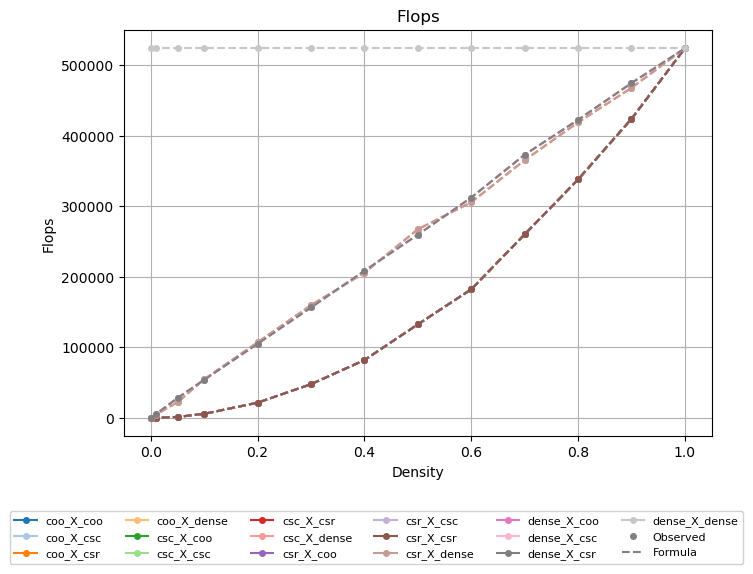
\includegraphics[width=\linewidth]{plots/plot_flops.png}
  \caption{Observed and Formula FLOPs. Observed data points fall mostly on the dotted line plotted from formulas.}
  \label{fig:flops}
\end{figure}

\begin{figure}[b]
  \centering
  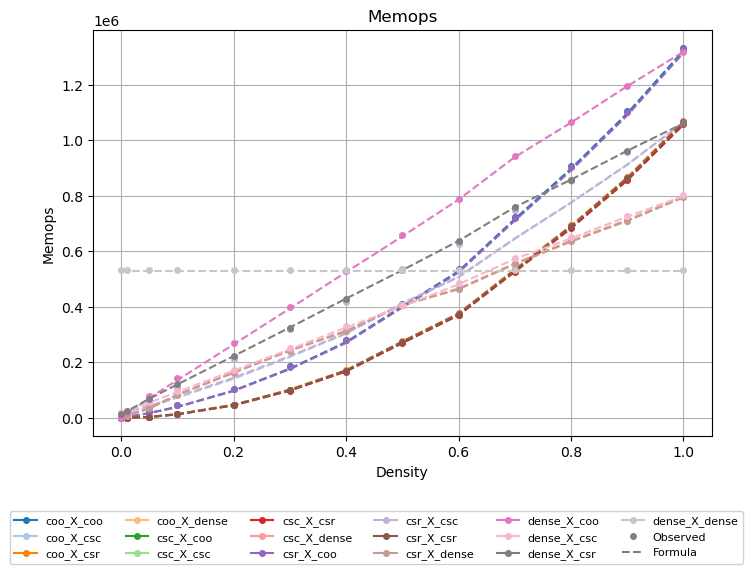
\includegraphics[width=\linewidth]{plots/plot_memops.png}
  \caption{Observed and Formula memops. Observed data points fall mostly on the dotted line plotted from formulas.}
  \label{fig:memops}
\end{figure}

\begin{figure}[t]
  \centering
  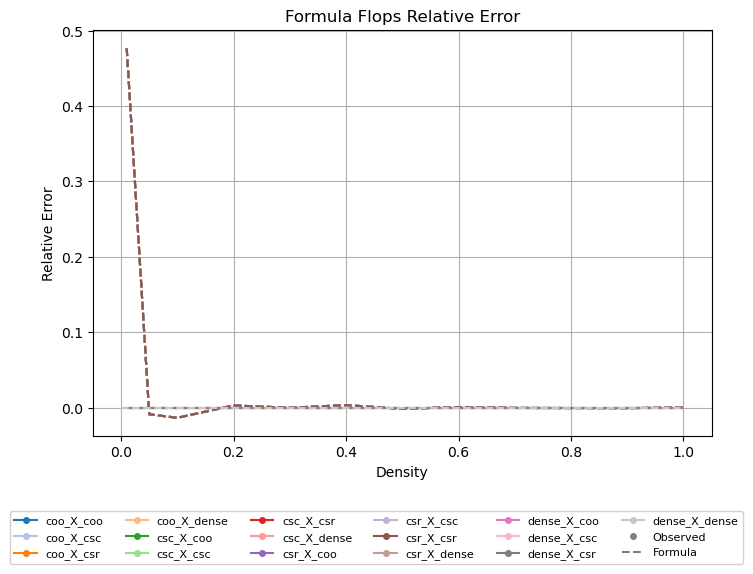
\includegraphics[width=\linewidth]{plots/plot_flop_error.png}
  \caption{FLOPs: Relative error of Formula vs Observed. Very close fit by the formula, and flop count is determined entirely by compression combination.}
  \label{fig:flop_error}
\end{figure}

\begin{figure}[b]
  \centering
  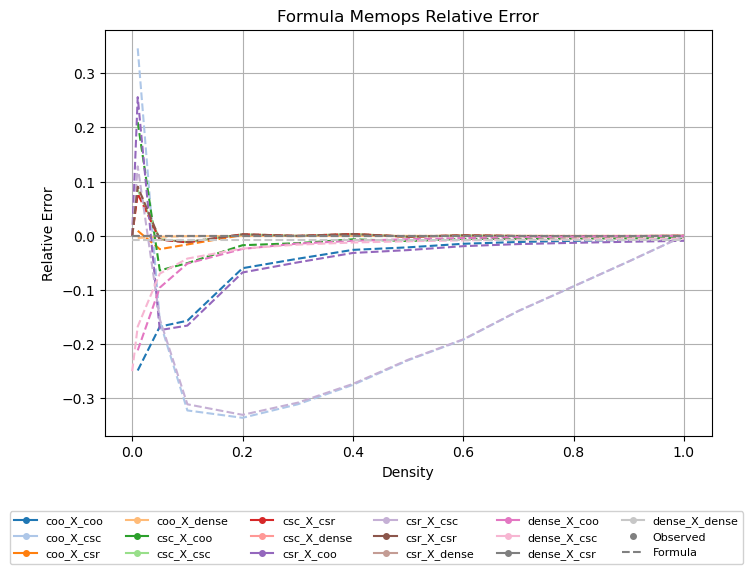
\includegraphics[width=\linewidth]{plots/plot_memop_error.png}
  \caption{memops: Relative error of Formula vs Observed. Close fit by most formulas, variability due to the effect of variability of sparsity patterns.}
  \label{fig:memop_error}
\end{figure}

\begin{figure}[t]
  \centering
  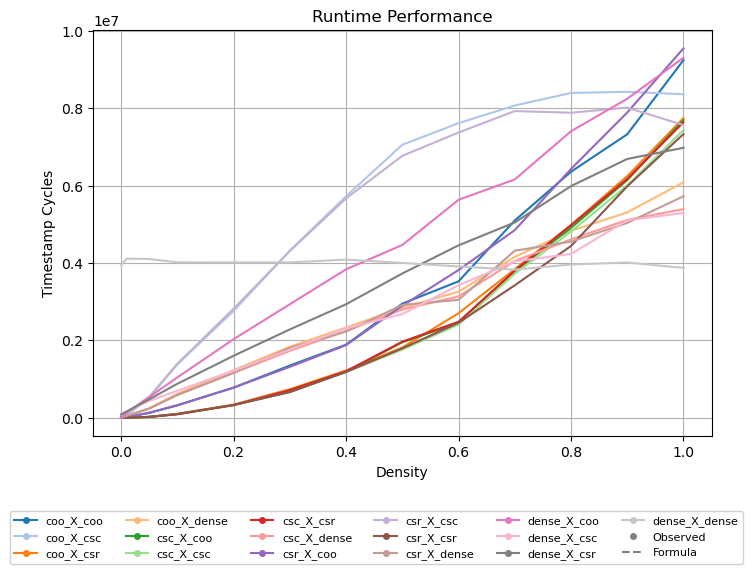
\includegraphics[width=\linewidth]{plots/plot_time.png}
  \caption{Runtime Performance: Timestamp Cycles. Crossover points at 0.7\% density when performing a simple dense x dense is better.}
  \label{fig:time}
\end{figure}

\begin{figure}[b]
  \centering
  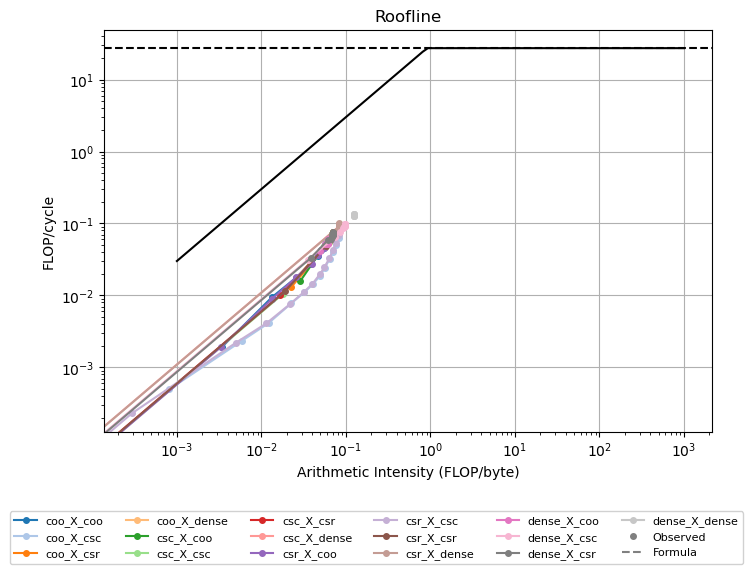
\includegraphics[width=\linewidth]{plots/plot_roofline.png}
  \caption{Roofline Model. Sparse formats are entirely memory bound.}
  \label{fig:roofline}
\end{figure}

\subsection{Format Selection Optimization Results}
An important finding concerns the cost model used to drive the format selection.
The analytical formulae derived in Section 3.2, while accurate predictors of operation counts,
proved to be poor proxies for actual runtime when used directly as the solver objective.
Format assignments produced using the formula-based cost model were outperformed by
assignments produced using empirically measured cycle counts from the density sweep as
the cost function. This suggests that operation count alone is an insufficient proxy for
runtime at this block size, likely because cache effects and branch misprediction dominate
over raw arithmetic and memory operation counts for 32×32 blocks. In essence,
our formulas mistakenly treat flops and memops as being comparable on their face, when
they are not. The formulas could perhaps become more predictive at larger block sizes
where compute cost dominates over fixed per-block overheads.

\begin{figure}[t]
  \centering
  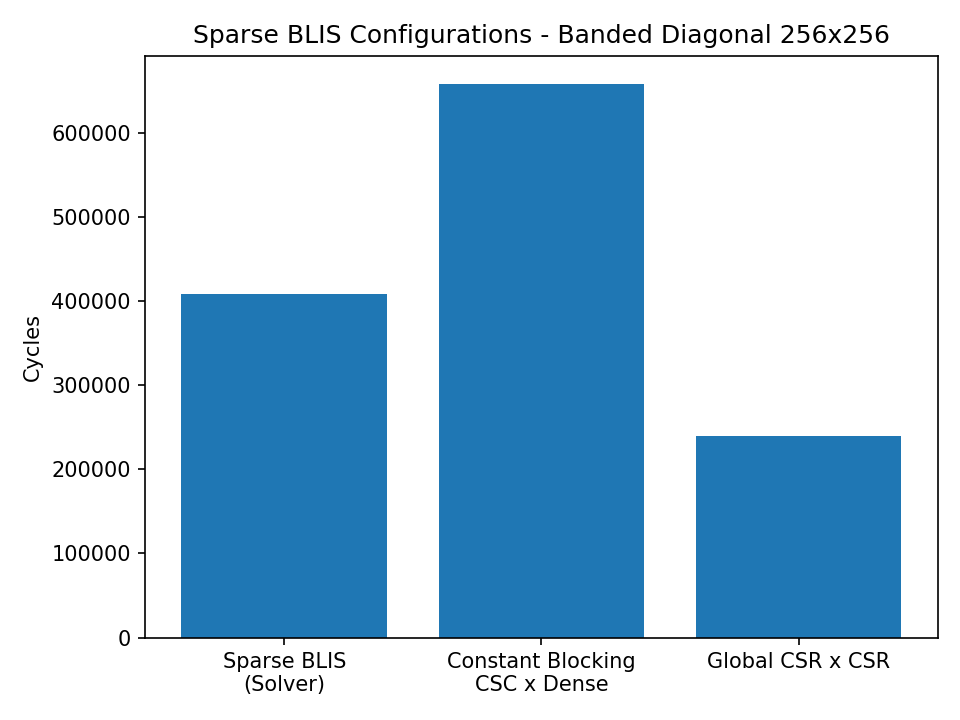
\includegraphics[width=\linewidth]{plots/diagonal_results.png}
  \caption{Diagonal Matrix Results. Poor performance compared to simple global compression, but optimal micro-format selection wins over naive format selection.}
  \label{fig:diagonal}
\end{figure}

Figure \ref{fig:diagonal} shows the performance of the three configurations on a synthetic banded
diagonal 256×256 matrix, the most favorable case for heterogeneous format selection as
it exhibits clear density variation between diagonal and off-diagonal blocks.
Even here, the solver-assigned configuration requires 408,725 cycles, compared to
239,189 cycles for global CSR x CSR, a 41\% gap. The constant blocking configuration
performs worst at 658,040 cycles, suggesting that solver assignment does at
least select better formats than a naive uniform choice in this case, but neither blocking
approach approaches the performance of the flat global baseline, unfortunately.

Figure 9 shows thread scaling. Performance does not improve meaningfully with additional threads and degrades at 8 threads, indicating the workload is too small and too irregular to benefit from parallelism at this scale.

Figure 10 shows the Kronecker graph sweep. Sparse BLIS scales poorly with matrix size while global CSR×CSR remains effectively flat, reflecting that block dispatch overhead grows with the number of blocks while the actual sparse compute remains minimal due to the uniformly low density of Kronecker graph matrices.

\subsubsection{Blocking Sensitivity}
\begin{figure}[t]
  \centering
  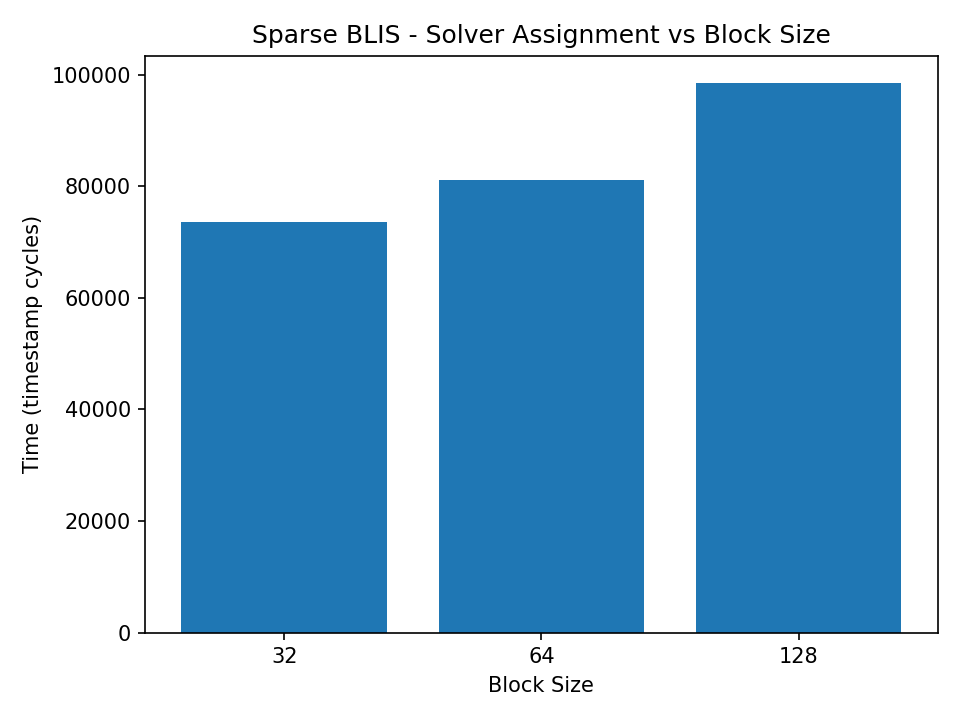
\includegraphics[width=\linewidth]{plots/block_size_sweep.png}
  \caption{Block Size Performance Impact. Performance degrades as block sizes increase.}
  \label{fig:block_size}
\end{figure}

Figure \ref{fig:block_size} shows performance across block sizes of 32, 64, and 128. Cycle count increases
with block size, likely due to increased cache pressure from the growing dense
accumulation buffer and greater work per block pair in the inner loop nest.

\subsubsection{Thread Sensitivity}
\begin{figure}[b]
  \centering
  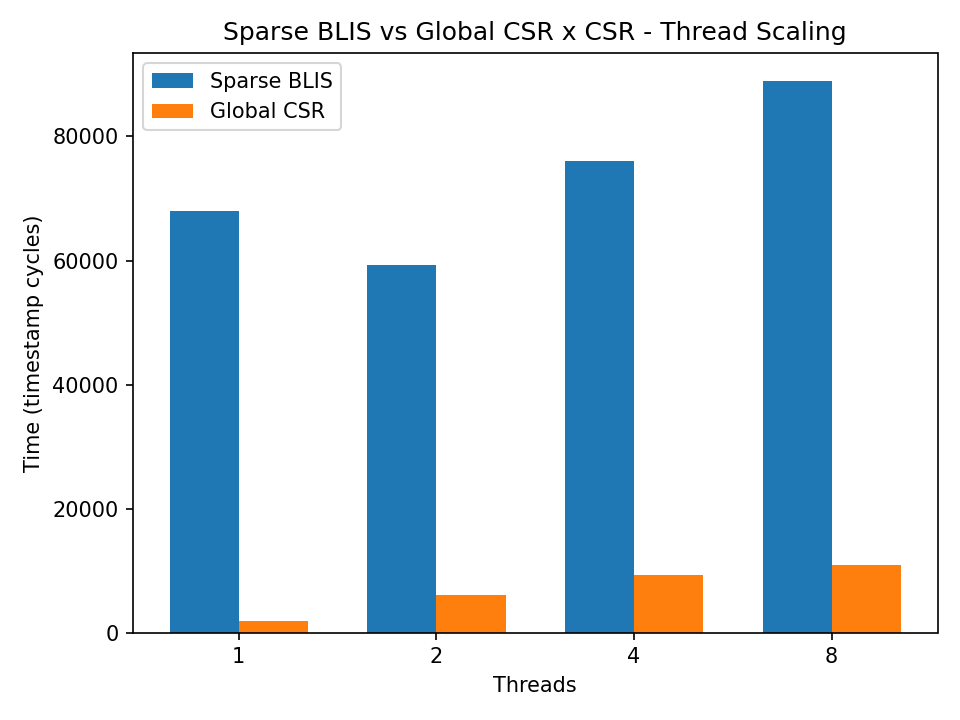
\includegraphics[width=\linewidth]{plots/thread_scaling.png}
  \caption{Thread Count Performance Impact. At matrix sizes that can be solved, threading provides minimal benefit beyond 2 threads.}
  \label{fig:threads}
\end{figure}

Figure \ref{fig:threads} shows thread scaling. Performance does not improve
meaningfully with additional threads and degrades at 8 threads, indicating the
workload is too small and too irregular to benefit from parallelism at this scale.

\subsection{Kronecker Graph Results}
\begin{figure}[t]
  \centering
  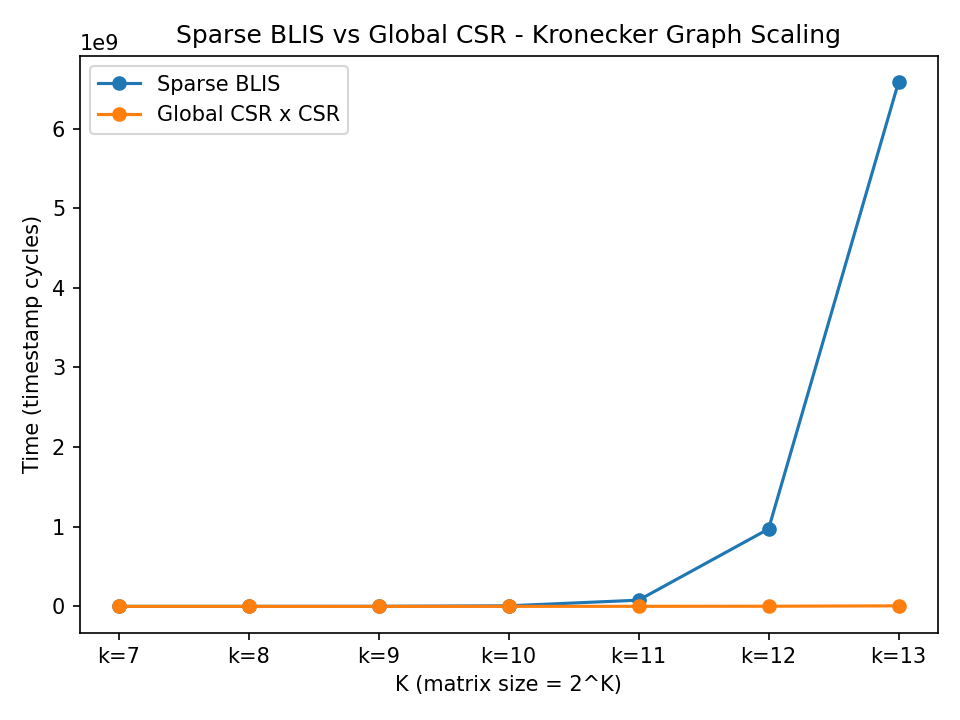
\includegraphics[width=\linewidth]{plots/kronecker_scaling.png}
  \caption{Kronecker Graph Sweep (AS-Newman). Sparse BLIS performs very poorly compared to a global compression strategy, this worsens as matrix size increases.}
  \label{fig:kron}
\end{figure}

\begin{figure}[b]
  \centering
  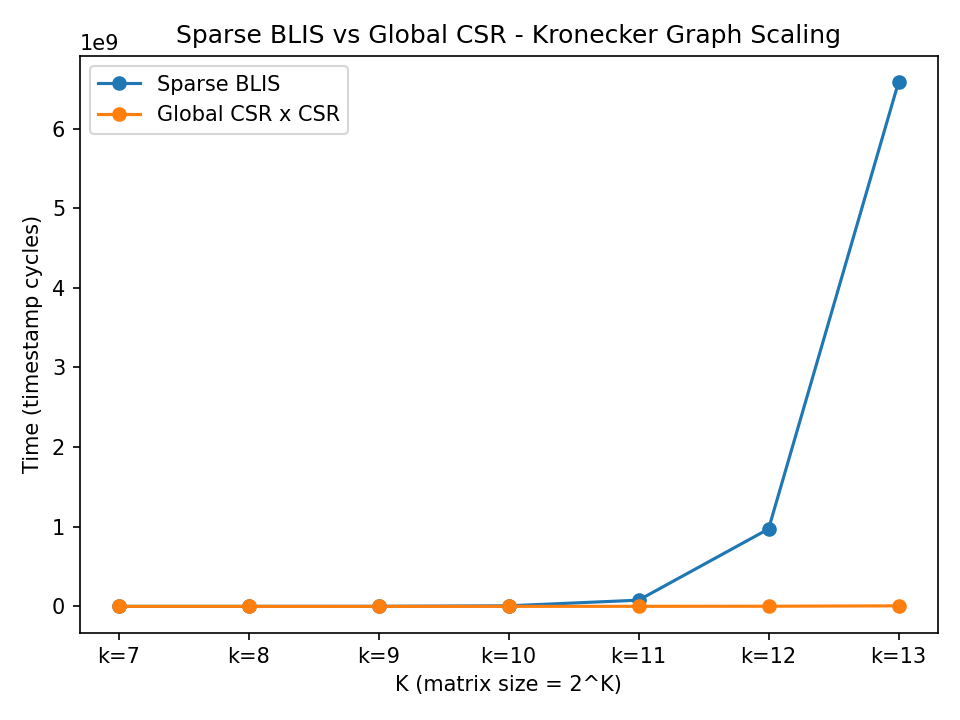
\includegraphics[width=\linewidth]{plots/kronecker_scaling.png}
  \caption{Kronecker Graph Sweep (AS-Newman). Sparse BLIS performs very poorly compared to a global compression strategy, this worsens as matrix size increases.}
  \label{fig:kron}
\end{figure}

\begin{figure}[t]
  \centering
  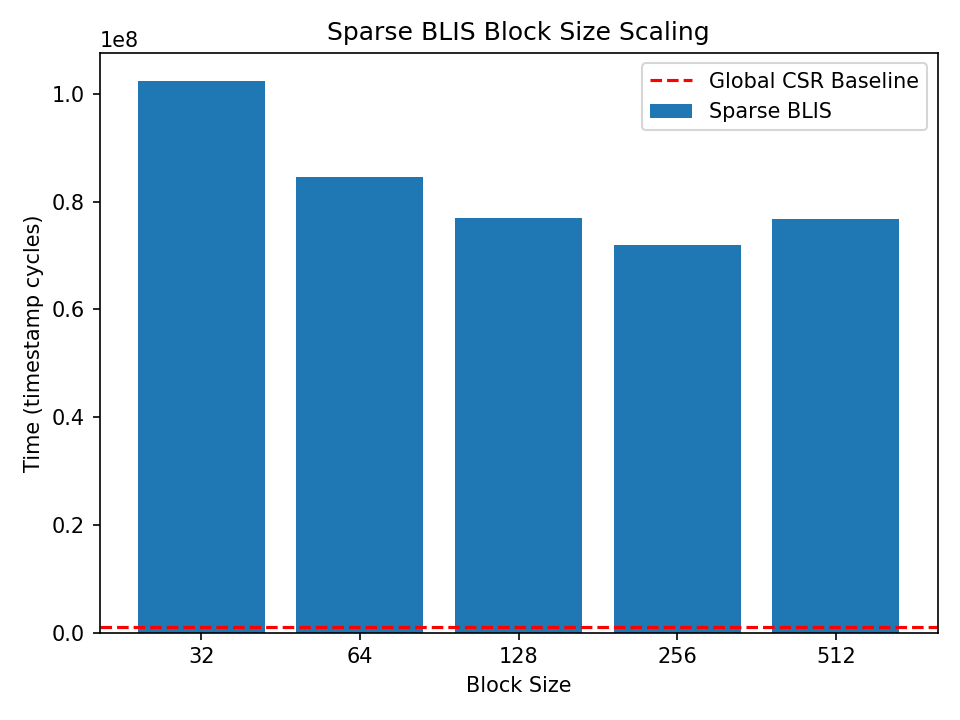
\includegraphics[width=\linewidth]{plots/kron_block_scaling.png}
  \caption{Kronecker Graph k=10 (AS-Newman) block size sweep. Block dispatch overhead generally decreases as block size increases, but not nearly enough to be comparable to simple global compression.}
  \label{fig:kron_blocks}
\end{figure}

Figure \ref{fig:kron} shows the Kronecker graph sweep. Sparse BLIS scales poorly with
matrix size while global CSRxCSR remains effectively flat, reflecting that block
dispatch overhead grows with the number of blocks while the actual sparse compute
remains minimal due to the uniformly low density of Kronecker graph matrices.

As noted in Section 3.5, the solver assigned a uniform CSCxCSR format to all
blocks for every Kronecker graph tested, collapsing the heterogeneous assignment to a
constant blocking scheme identical to the baseline. This confirms that the density
variation required to motivate mixed format selection is absent in these datasets.

Figure \ref{fig:kron_blocks} presents a sweep over progressively larger block sizes for Sparse BLIS. While the conventional micro-block dimension is $32\times32$, this experiment extends into block sizes that can no longer be strictly classified as micro-blocks. Nevertheless, even at these larger granularities, the additional blocking overhead proves insufficient to overcome the inherent inefficiencies, at least for this dataset.

\section{Summary}

We presented a study of SpGEMM across all sixteen pairings of four sparse matrix
storage formats, deriving analytical formulas for floating-point and memory operation
counts that show strong agreement with empirically measured values for fourteen of the
sixteen combinations.

Building on these formulas, we implemented a BLIS-inspired~\cite{blis} sparse matrix
multiplication pipeline that assigns storage formats independently to each micro-block
and dispatches to the corresponding kernel at runtime. Format selection is formulated
as a MINLP and solved using Pyomo~\cite{pyomo} with MindtPy~\cite{mindtpy}. Evaluation
on banded diagonal matrices and Kronecker graph datasets~\cite{kronecker} shows that
block dispatch overhead consistently dominates runtime, preventing the heterogeneous
approach from matching a flat global CSR$\times$CSR baseline despite producing better
format choices than a naive uniform assignment.

Several directions could address these limitations. A more uniform blocking/adaptable
format for the inner most microblocks could be explored. A lighter-weight greedy format
selection heuristic, rather than a full MINLP solve, could reduce planning overhead.
Finally, the approach could be better suited to architectures with less penalty for very
branch-y inner loops.

\bibliographystyle{ACM-Reference-Format}
\bibliography{references}

\end{document}
\endinput
